\chapter{Verwendete Technologien}
\label{Verwendete Technologien}

\section{Angular 2}
Es gibt unzählige Frameworks und Technologien für die Webentwicklung mit Java\-Script. Die weite Verbreitung von dem Platzhirsch \emph{AngularJS} kann beispielsweise durch die Anzahl an mit dem Tag "`angularjs"' versehenen Fragen auf \texttt{stackoverflow.com} belegt werden. Januar 2017 sind es 213 992 Fragen. Im Vergleich dazu sind 20 343 Fragen mit einem entsprechendem \emph{Ember.js} Tag versehen und bei dem immer beliebter werdenden Framework \emph{React.js} von \emph{Facebook} sind es immerhin 30 222 \cite{stackoverflow}.

Angular (oder auch AngularJS) ist ein seit 2009 von Google Inc. entwickeltes Framework und Open-Source-Projekt für Single-Page-Applicationen, d.h. Applikationen, die nur aus einer einzelnen HTML-Seite bestehen und deren Inhalte dynamisch nachgeladen werden. Die Sofwareentwicklung mit Angular wird im Gegensatz zu Softwareentwicklung mit reinem JavaScript deutlich vereinfacht, indem dem Entwickler Strukturen und Bibliotheken vorgegeben und Entscheidungen abgenommen werden. Mit dem Model-View-ViewModel unterstützt Angular bidirektionales Databinding.

Seit 2015 wird Angular 2 entwickelt und die zugrunde liegende Architektur von Angular wurde in diesem Zuge komplett überarbeitet. Angular 2 ist somit auch nicht mehr zu Angular 1 kompatibel. Der offensichtlichste Unterschied zu Angular 1 ist die Sprache in der Angular 2 geschrieben ist. Es wurde auf den Javascript Aufsatz TypeScript gesetzt. Dieser wurde von Microsoft entwickelt und erweitert JavaScript um die Möglichkeit objektorientiert und typsicher zu programmieren. TypeScript kann zu nativem JavaScript transpiliert werden.

Weiterhin ist Angular 2 Komponenten-orientiert. Das bedeutet, dass eine Applikation in beliebig viele kleine Komponenten aufgeteilt werden können, die durch gekapselte Logik und Wiederverwendbarkeit geprägt sind. Jede Komponente besteht aus einem Template in HTML, einer zugehörigen Klasse in Typescript und Sytlesheets in CSS oder mithilfe von CSS-Präprozessoren wie SASS oder LESS.

Eine \texttt{HelloWorld}-Komponente würde in Angular 2 folgendermaßen aussehen:
\begin{codebox}
\begin{lstlisting}[style=typescript]
import {Component} from '@angular/core';

@Component({
  selector: 'hello-world',
  template: '<p>Hello world!</p>',
  styles: ['p {color: red}']
})
export class HelloWorldComponent {
}
\end{lstlisting}
\end{codebox}

Template und Styles würden in einer Komponente eines echten Projekts der besseren Wartbarkeit halber noch in einzelne Dokumente ausgelagert werden.

Diese \texttt{HelloWorld}-Komponente könnte dann in einer Eltern-Komponente mit
\begin{codebox}
\begin{lstlisting}[language=HTML]
<hello-world></hello-world>
\end{lstlisting}
\end{codebox}
eingebunden werden.

\section{Cordova}

Cordova ist eine Open-Source-Framework für die Entwicklung mobiler Applikationen mit den Standard Webtechnologien HTML5, CSS und JavaScript (vgl. \cite{cordova}).

\begin{figure}[htb]
\centering
\caption{Cordova Architektur}
\label{fig:netzabdeckung}
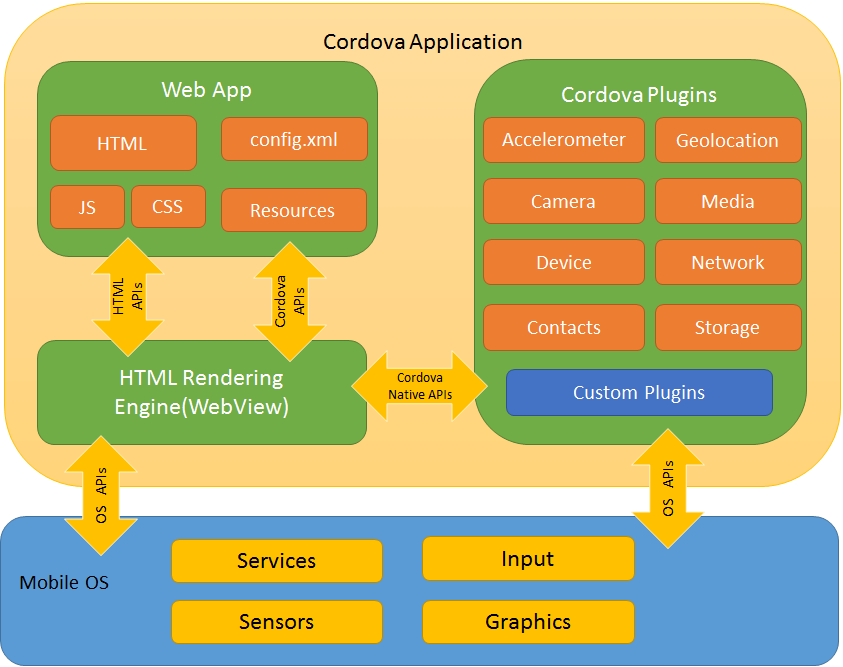
\includegraphics[width=0.8\textwidth]{\figdir/cordova.png}
\end{figure}

\section{Ionic}












